\documentclass[11pt,a4paper]{report}
\usepackage[textwidth=37em,vmargin=30mm]{geometry}
\usepackage{calc,xunicode,amsmath,amssymb,paralist,enumitem,tabu,booktabs,datetime2,xeCJK,xeCJKfntef,listings}
\usepackage{tocloft,fancyhdr,tcolorbox,xcolor,graphicx,eso-pic,xltxtra,xelatexemoji}

\newcommand{\envyear}[0]{2025}
\newcommand{\envdatestr}[0]{2025-09-01}
\newcommand{\envfinaldir}[0]{webdb/2025/20250901/final}

\usepackage[hidelinks]{hyperref}
\hypersetup{
    colorlinks=false,
    pdfpagemode=FullScreen,
    pdftitle={Web Digest - \envdatestr}
}

\setlength{\cftbeforechapskip}{10pt}
\renewcommand{\cftchapfont}{\rmfamily\bfseries\large\raggedright}
\setlength{\cftbeforesecskip}{2pt}
\renewcommand{\cftsecfont}{\sffamily\small\raggedright}

\setdefaultleftmargin{2em}{2em}{1em}{1em}{1em}{1em}

\usepackage{xeCJK,xeCJKfntef}
\xeCJKsetup{PunctStyle=plain,RubberPunctSkip=false,CJKglue=\strut\hskip 0pt plus 0.1em minus 0.05em,CJKecglue=\strut\hskip 0.22em plus 0.2em}
\XeTeXlinebreaklocale "zh"
\XeTeXlinebreakskip = 0pt


\setmainfont{Brygada 1918}
\setromanfont{Brygada 1918}
\setsansfont{IBM Plex Sans}
\setmonofont{JetBrains Mono NL}
\setCJKmainfont{Noto Serif CJK SC}
\setCJKromanfont{Noto Serif CJK SC}
\setCJKsansfont{Noto Sans CJK SC}
\setCJKmonofont{Noto Sans CJK SC}

\setlength{\parindent}{0pt}
\setlength{\parskip}{8pt}
\linespread{1.15}

\lstset{
	basicstyle=\ttfamily\footnotesize,
	numbersep=5pt,
	backgroundcolor=\color{black!5},
	showspaces=false,
	showstringspaces=false,
	showtabs=false,
	tabsize=2,
	captionpos=b,
	breaklines=true,
	breakatwhitespace=true,
	breakautoindent=true,
	linewidth=\textwidth
}






\newcommand{\coverpic}[2]{
    % argv: itemurl, authorname
    Cover photo by #2~~(\href{#1}{#1})
}
\newcommand{\makeheader}[0]{
    \begin{titlepage}
        % \newgeometry{hmargin=15mm,tmargin=21mm,bmargin=12mm}
        \begin{center}
            
            \rmfamily\scshape
            \fontspec{BaskervilleF}
            \fontspec{Old Standard}
            \fontsize{59pt}{70pt}\selectfont
            WEB\hfill DIGEST
            
            \vfill
            % \vskip 30pt
            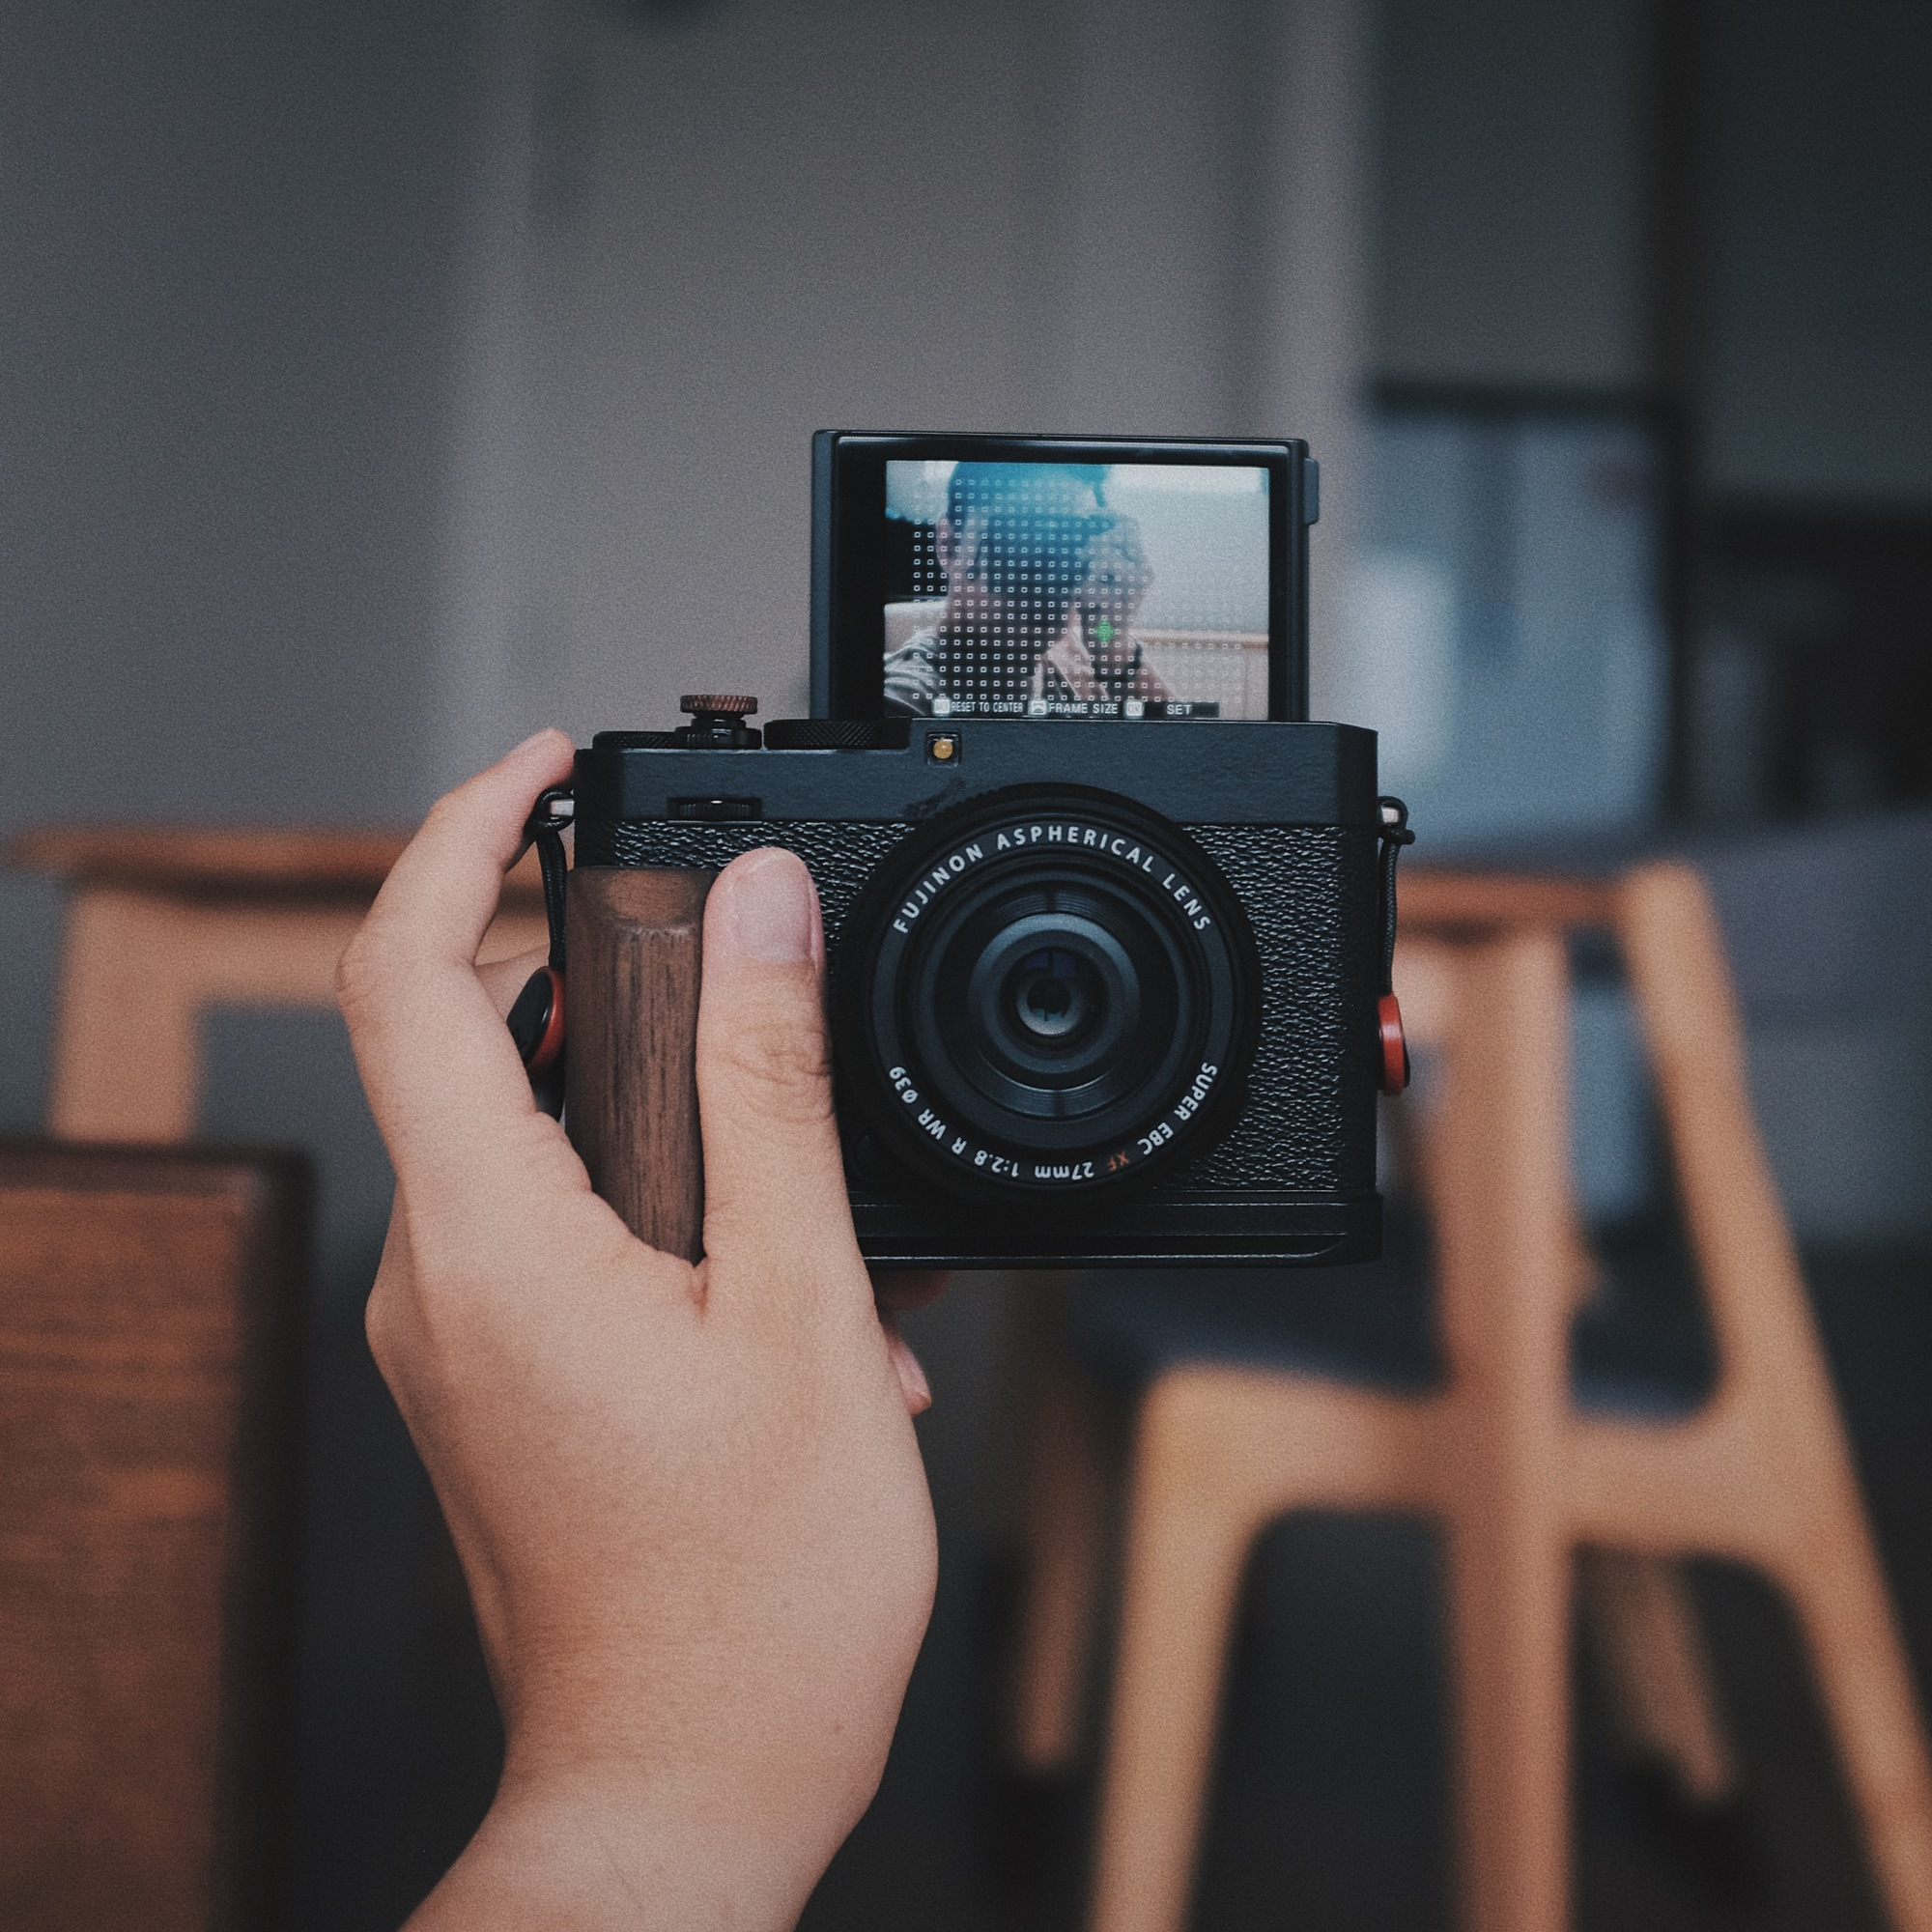
\includegraphics[width=\linewidth]{\envfinaldir/coverpic-prod.jpg}\par
            % \vskip 30pt
            \vfill

            \normalsize\rmfamily\scshape
            \copyright{} The Web Digest Project \hfill\large \envdatestr
        \end{center}
    \end{titlepage}
    % \restoregeometry
}
\newcommand{\simplehref}[1]{%
    \textcolor{blue!80!green}{\href{#1}{#1}}%
}
\renewcommand{\contentsname}{\center\Huge\sffamily\bfseries Contents\par\vskip 20pt}
\newcounter{ipartcounter}
\setcounter{ipartcounter}{0}
\newcommand{\ipart}[1]{
    % \vskip 20pt
    \clearpage
    \stepcounter{ipartcounter}
    \phantomsection
    \addcontentsline{toc}{chapter}{#1}
    % \begin{center}
    %     \Huge
    %     \sffamily\bfseries
    %     #1
    % \end{center}
    % \vskip 20pt plus 7pt
}
\newcounter{ichaptercounter}
\setcounter{ichaptercounter}{0}
\newcommand{\ichapter}[1]{
    % \vskip 20pt
    \clearpage
    \stepcounter{ichaptercounter}
    \phantomsection
    \addcontentsline{toc}{section}{\numberline{\arabic{ichaptercounter}}#1}
    \begin{center}
        \Huge
        \sffamily\bfseries
        #1
    \end{center}
    \vskip 20pt plus 7pt
}
\newcommand{\entrytitlefont}[1]{\subsection*{\raggedright\Large\sffamily\bfseries#1}}
\newcommand{\entryitemGeneric}[2]{
    % argv: title, url
    \parbox{\linewidth}{
        \entrytitlefont{#1}\par\vskip 5pt
        \footnotesize\ttfamily\mdseries
        \simplehref{#2}
    }\vskip 11pt plus 11pt minus 1pt
}
\newcommand{\entryitemGithub}[3]{
    % argv: title, url, desc
    \parbox{\linewidth}{
        \entrytitlefont{#1}\par\vskip 5pt
        \footnotesize\ttfamily\mdseries
        \simplehref{#2}\par\vskip 5pt
        \small\rmfamily\mdseries#3
    }\vskip 11pt plus 11pt minus 1pt
}
\newcommand{\entryitemAp}[3]{
    % argv: title, url, desc
    \parbox{\linewidth}{
        \entrytitlefont{#1}\par\vskip 5pt
        \footnotesize\ttfamily\mdseries
        \simplehref{#2}\par\vskip 5pt
        \small\rmfamily\mdseries#3
    }\vskip 11pt plus 11pt minus 1pt
}
\newcommand{\entryitemHackernews}[3]{
    % argv: title, hnurl, rawurl
    % \parbox{\linewidth}{
    %     \entrytitlefont{#1}\par\vskip 5pt
    %     \footnotesize\ttfamily\mdseries
    %     \simplehref{#3}\par
    %     \textcolor{black!50}{\href{#2}{#2}}
    % }\vskip 11pt plus 11pt minus 1pt
    \begin{minipage}{\linewidth}
            \entrytitlefont{#1}\par\vskip 5pt
            \footnotesize\ttfamily\mdseries
            \simplehref{#3}\par
            \textcolor{black!50}{\href{#2}{#2}}
    \end{minipage}\par\vskip 11pt plus 11pt minus 1pt
}







\begin{document}

\makeheader

\tableofcontents\clearpage




\ipart{Developers}
\ichapter{Hacker News}
\entryitemTwoLinks{Eternal Struggle}{https://news.ycombinator.com/item?id=45086020}{https://yoavg.github.io/eternal/}

\entryitemTwoLinks{Use One Big Server (2022)}{https://news.ycombinator.com/item?id=45085029}{https://specbranch.com/posts/one-big-server/}

\entryitemTwoLinks{Ask HN: How do you fight YouTube addiction and procrastination? I'm struggling}{https://news.ycombinator.com/item?id=45085014}{https://news.ycombinator.com/item?id=45085014}

\entryitemTwoLinks{When the sun will literally set on what's left of the British Empire}{https://news.ycombinator.com/item?id=45084913}{https://oikofuge.com/sun-sets-on-british-empire/}

\entryitemTwoLinks{I Don't Have Spotify}{https://news.ycombinator.com/item?id=45084673}{https://idonthavespotify.sjdonado.com/}

\entryitemTwoLinks{No clicks, no content: The unsustainable future of AI search}{https://news.ycombinator.com/item?id=45084016}{https://bradt.ca/blog/no-clicks-no-content/}

\entryitemTwoLinks{Jujutsu for Everyone}{https://news.ycombinator.com/item?id=45083952}{https://jj-for-everyone.github.io/}

\entryitemTwoLinks{FDA official demands removal of YouTube videos of himself criticizing vaccines}{https://news.ycombinator.com/item?id=45083845}{https://www.theguardian.com/us-news/2025/aug/31/fda-official-youtube-videos}

\entryitemTwoLinks{Notes on Managing ADHD}{https://news.ycombinator.com/item?id=45083134}{https://borretti.me/article/notes-on-managing-adhd}

\entryitemTwoLinks{Google: 'Your \$1000 phone needs our permission to install apps now' [video]}{https://news.ycombinator.com/item?id=45082750}{https://www.youtube.com/watch?v=QBEKlIV\_70E}

\entryitemTwoLinks{``This telegram must be closely paraphrased before being communicated to anyone''}{https://news.ycombinator.com/item?id=45082731}{https://history.stackexchange.com/questions/79371/this-telegram-must-be-closely-paraphrased-before-being-communicated-to-anyone}

\entryitemTwoLinks{F-Droid site certificate expired}{https://news.ycombinator.com/item?id=45082595}{https://gitlab.com/fdroid/fdroid-website/-/issues/883}

\entryitemTwoLinks{Why haven't quantum computers factored 21 yet?}{https://news.ycombinator.com/item?id=45082587}{https://algassert.com/post/2500}

\entryitemTwoLinks{Git Diagramming "The Weave"}{https://news.ycombinator.com/item?id=45080720}{https://daverupert.com/2025/08/git-diagramming-the-weave/}

\entryitemTwoLinks{Rick Beato is right to rant about music copyright strikes}{https://news.ycombinator.com/item?id=45080618}{https://savingcountrymusic.com/rick-beato-is-right-to-rant-about-music-copyright-strikes/}

\entryitemTwoLinks{My phone is an ereader now}{https://news.ycombinator.com/item?id=45079962}{https://www.davepagurek.com/blog/minimal-phone/}

\entryitemTwoLinks{Are people's bosses making them use AI tools?}{https://news.ycombinator.com/item?id=45079911}{https://piccalil.li/blog/are-peoples-bosses-really-making-them-use-ai/}

\entryitemTwoLinks{Affiliates flock to scam gambling machine}{https://news.ycombinator.com/item?id=45078530}{https://krebsonsecurity.com/2025/08/affiliates-flock-to-soulless-scam-gambling-machine/}

\entryitemTwoLinks{Six months into tariffs, businesses have no idea how to price anything}{https://news.ycombinator.com/item?id=45077937}{https://www.wsj.com/business/retail/trump-tariff-business-price-impact-37b630c8}

\entryitemTwoLinks{Why did books start being divided into chapters? A new history}{https://news.ycombinator.com/item?id=45077735}{https://sydneyreviewofbooks.com/reviews/just-a-little-longer}


\ipart{Developers~~~~(zh-Hans)}
\ichapter{Solidot}
\entryitemGeneric{\hskip 0pt{}Vivaldi 再次强调不会集成生成式 AI}{https://www.solidot.org/story?sid=82186}

\entryitemGeneric{\hskip 0pt{}美国国防部叫停了微软中国工程师参与的项目}{https://www.solidot.org/story?sid=82185}

\entryitemGeneric{\hskip 0pt{}FTC 指责 Gmail 过滤共和党筹款邮件威胁美国自由}{https://www.solidot.org/story?sid=82184}

\entryitemGeneric{\hskip 0pt{}Linus Torvalds 将 Bcachefs 标记为由外部维护}{https://www.solidot.org/story?sid=82183}

\entryitemGeneric{\hskip 0pt{}为平衡能耗和生存演化可能对大脑大小设置了上限}{https://www.solidot.org/story?sid=82182}

\entryitemGeneric{\hskip 0pt{}超加工食品可能是男性精子质量下降的一个原因}{https://www.solidot.org/story?sid=82181}

\entryitemGeneric{\hskip 0pt{}Valve 为遵守法律对访问成人内容的英国用户验证年龄}{https://www.solidot.org/story?sid=82180}

\entryitemGeneric{\hskip 0pt{}银河麒麟发布 V11,安装量达到 1600 万}{https://www.solidot.org/story?sid=82179}

\entryitemGeneric{\hskip 0pt{}良品铺子的 AI 广告显示花生长在树上}{https://www.solidot.org/story?sid=82177}

\entryitemGeneric{\hskip 0pt{}年轻人没有以前快乐了}{https://www.solidot.org/story?sid=82176}

\entryitemGeneric{\hskip 0pt{}美国将限制留学生和记者签证有效期}{https://www.solidot.org/story?sid=82175}

\entryitemGeneric{\hskip 0pt{}黄石公园内自由迁徙的野牛加强了草原的恢复力}{https://www.solidot.org/story?sid=82174}

\entryitemGeneric{\hskip 0pt{}美商务部长称将在区块链上发布经济数据}{https://www.solidot.org/story?sid=82173}

\entryitemGeneric{\hskip 0pt{}日本小镇考虑倡导每天仅使用智能手机两小时}{https://www.solidot.org/story?sid=82172}

\entryitemGeneric{\hskip 0pt{}FFmpeg 8 支持实时生成字幕}{https://www.solidot.org/story?sid=82171}

\entryitemGeneric{\hskip 0pt{}研究显示 AI 的普及与美国初级工作的减少相关}{https://www.solidot.org/story?sid=82170}\ichapter{V2EX}
\entryitemGeneric{\hskip 0pt{}[程序员] 为了魔改 chromium, 点满了各种技能树}{https://www.v2ex.com/t/1156130}

\entryitemGeneric{\hskip 0pt{}[问与答] 我们来一起做个实验吧}{https://www.v2ex.com/t/1156129}

\entryitemGeneric{\hskip 0pt{}[问与答] 公司内网邮箱不能用了, 如何将代码安全的传输到外部呢}{https://www.v2ex.com/t/1156128}

\entryitemGeneric{\hskip 0pt{}[反馈] @Livid 建议在创建新主题的校验规则中增加或条件``允许蓝钻、黄钻不满足注册时间条件''}{https://www.v2ex.com/t/1156126}

\entryitemGeneric{\hskip 0pt{}[电影] 豆瓣太恶心了!}{https://www.v2ex.com/t/1156125}

\entryitemGeneric{\hskip 0pt{}[问与答] 最近油管冒出个``淘淘****''总感觉是个 AI 主播}{https://www.v2ex.com/t/1156124}

\entryitemGeneric{\hskip 0pt{}[macOS] macOS 26 系统设置允许在菜单栏显示残留项目如何清理?}{https://www.v2ex.com/t/1156123}

\entryitemGeneric{\hskip 0pt{}[问与答] 请问 NAS SSD 主盘 + 自动 backup HDD 推荐}{https://www.v2ex.com/t/1156122}

\entryitemGeneric{\hskip 0pt{}[分享创造] AI 驱动的 web3 空投/活动聚合器}{https://www.v2ex.com/t/1156119}

\entryitemGeneric{\hskip 0pt{}[问与答] 求推荐 macbook}{https://www.v2ex.com/t/1156118}

\entryitemGeneric{\hskip 0pt{}[分享创造] 一个 ZIP 文件,解压后居然又包含自己,再解压还是自己……无限循环下去!😱}{https://www.v2ex.com/t/1156117}

\entryitemGeneric{\hskip 0pt{}[问与答] vibe coding or regular coding?}{https://www.v2ex.com/t/1156116}

\entryitemGeneric{\hskip 0pt{}[电动汽车] 来个 NIO 内部懂哥}{https://www.v2ex.com/t/1156115}

\entryitemGeneric{\hskip 0pt{}[旅行] 东京两周生活初印象:优点篇(纯主观)}{https://www.v2ex.com/t/1156114}

\entryitemGeneric{\hskip 0pt{}[NAS] 现在 1u(长度 40cm 以内),全闪, 8*nvme/8*e1.s/4*u2 热插拔,单路 NAS 有啥作业可以抄么}{https://www.v2ex.com/t/1156113}

\entryitemGeneric{\hskip 0pt{}[问与答] 不知道各位老哥有没有发现公交车班次变少了}{https://www.v2ex.com/t/1156111}

\entryitemGeneric{\hskip 0pt{}[程序员] vibe coding 一点也不 vibe}{https://www.v2ex.com/t/1156110}

\entryitemGeneric{\hskip 0pt{}[OpenAI] ChatGPT Plus 订阅了两年,手头紧有什么平替方案}{https://www.v2ex.com/t/1156109}

\entryitemGeneric{\hskip 0pt{}[Solana] 疯狂的一周}{https://www.v2ex.com/t/1156108}

\entryitemGeneric{\hskip 0pt{}[程序员] Cherry Studio + MCP Server 我们还需要前端吗}{https://www.v2ex.com/t/1156106}

\entryitemGeneric{\hskip 0pt{}[生活] 有没有天津南开区的 v 友能帮忙转寄下国补快递}{https://www.v2ex.com/t/1156105}

\entryitemGeneric{\hskip 0pt{}[问与答] 千元以内给电脑的有源音箱有能打的吗?}{https://www.v2ex.com/t/1156104}

\entryitemGeneric{\hskip 0pt{}[Solana] 20250831 - Cold Wallet 操作说明}{https://www.v2ex.com/t/1156103}

\entryitemGeneric{\hskip 0pt{}[问与答] 公众号文章如何导出到网站正常访问}{https://www.v2ex.com/t/1156102}

\entryitemGeneric{\hskip 0pt{}[Apple] ios 自签的音乐视频软件无法使用空间音频}{https://www.v2ex.com/t/1156101}

\entryitemGeneric{\hskip 0pt{}[分享创造] 🎉 极简易用的 Mac 剪贴板增强工具「AegisClip」官网上线啦!}{https://www.v2ex.com/t/1156100}

\entryitemGeneric{\hskip 0pt{}[程序员] 世界是一个巨大的草台班子?还是这是 Linux 系统的什么古老传统?}{https://www.v2ex.com/t/1156099}

\entryitemGeneric{\hskip 0pt{}[macOS] MacOS 下,浏览器观看视频双击最大化菜单栏问题}{https://www.v2ex.com/t/1156096}

\entryitemGeneric{\hskip 0pt{}[Solana] 我的 Solana 手机 SEEKER 终于到了}{https://www.v2ex.com/t/1156095}

\entryitemGeneric{\hskip 0pt{}[分享创造] vibe coding 了一个 AI 实战社区网站,邀请有兴趣的同学上线测试}{https://www.v2ex.com/t/1156094}

\entryitemGeneric{\hskip 0pt{}[Solana] 有人能分享一下 web3 空投收益有多少?}{https://www.v2ex.com/t/1156093}

\entryitemGeneric{\hskip 0pt{}[游戏] 如果游戏全上云理论上是不是就杜绝外挂了}{https://www.v2ex.com/t/1156092}

\entryitemGeneric{\hskip 0pt{}[分享发现] 越南 Viettel 电话卡}{https://www.v2ex.com/t/1156091}

\entryitemGeneric{\hskip 0pt{}[酷工作] 招聘(远程办公, Web3): Rust \& C++ 交易系统, 前端, Golang(5+ HC), Flutter, 日本区社群运营负责人, Seo 优化师, 视觉设计师, 合约测试开发, 北美市场负责人、欧洲市场负责人}{https://www.v2ex.com/t/1156090}

\entryitemGeneric{\hskip 0pt{}[云计算] Ucloud 台湾机房体验爆炸,十几天售后相互推诿}{https://www.v2ex.com/t/1156085}

\entryitemGeneric{\hskip 0pt{}[问与答] 问下各位:到底是电车好还是油车好?}{https://www.v2ex.com/t/1156084}

\entryitemGeneric{\hskip 0pt{}[推广] V 友们保真包甜包脆赛过初恋的大荔冬枣考虑一下~~}{https://www.v2ex.com/t/1156082}

\entryitemGeneric{\hskip 0pt{}[路由器] 为什么无论什么路由器,网友都会说:疯狂断流}{https://www.v2ex.com/t/1156081}

\entryitemGeneric{\hskip 0pt{}[随想] ai 技术对人类语言表达和思维方式的影响}{https://www.v2ex.com/t/1156079}

\entryitemGeneric{\hskip 0pt{}[全球工单系统] 朋友们的 22 端口还好么?}{https://www.v2ex.com/t/1156078}

\entryitemGeneric{\hskip 0pt{}[分享创造] 他们到底在吵什么}{https://www.v2ex.com/t/1156077}

\entryitemGeneric{\hskip 0pt{}[分享创造] 娃终于上幼儿园了,腾出时间做了个单词拼写小游戏网站 outspell word game}{https://www.v2ex.com/t/1156074}

\entryitemGeneric{\hskip 0pt{}[分享发现] 零成本搭建功能完善的论坛!}{https://www.v2ex.com/t/1156073}

\entryitemGeneric{\hskip 0pt{}[问与答] 武汉宽带套餐求推荐}{https://www.v2ex.com/t/1156072}

\entryitemGeneric{\hskip 0pt{}[分享发现] Grok 生成视频有点意思,我尝试生成日本少女}{https://www.v2ex.com/t/1156071}

\entryitemGeneric{\hskip 0pt{}[分享创造] 跟热点做了个 Nano Banana 网站,发现完全拿不到流量,那就改成完全免费的吧}{https://www.v2ex.com/t/1156070}

\entryitemGeneric{\hskip 0pt{}[问与答] iPhone 当作妙控板}{https://www.v2ex.com/t/1156068}

\entryitemGeneric{\hskip 0pt{}[宽带症候群] 华为 FTTR F30(光猫路由一体)是不是局域网设备不能看组播 IPTV?}{https://www.v2ex.com/t/1156066}

\entryitemGeneric{\hskip 0pt{}[分享创造] 开源热榜聚合 API 服务,增加了定时抓取数据源保存数据的功能,方便查询历史热点数据}{https://www.v2ex.com/t/1156063}

\entryitemGeneric{\hskip 0pt{}[问与答] 请问,微信小程序的激励广告,现在收益如何呢?}{https://www.v2ex.com/t/1156062}


\ipart{Generic News}







\clearpage
\leavevmode\vfill
\footnotesize

Copyright \copyright{} 2023-2025 Neruthes and other contributors.

This document is published with CC BY-NC-ND 4.0 license.

The entries listed in this newsletter may be copyrighted by their respective creators.

This newsletter is generated by the Web Digest project.

The newsletters are also delivered via Telegram channel \CJKunderline{\href{https://t.me/webdigestchannel}{https://t.me/webdigestchannel}}.\\
RSS feed is available at \CJKunderline{\href{https://webdigest.pages.dev/rss.xml}{https://webdigest.pages.dev/rss.xml}}.

This newsletter is available in PDF at
\CJKunderline{\href{https://webdigest.pages.dev/}{https://webdigest.pages.dev/}}.

The source code being used to generate this newsletter is available at\\
\CJKunderline{\href{https://github.com/neruthes/webdigest}{https://github.com/neruthes/webdigest}}.

This newsletter is also available in
\CJKunderline{\href{http://webdigest.pages.dev/readhtml/\envyear/WebDigest-20250901.html}{HTML}} and
\CJKunderline{\href{https://github.com/neruthes/webdigest/blob/master/markdown/\envyear/WebDigest-20250901.md}{Markdown}}.


\coverpic{https://unsplash.com/photos/people-in-blue-dresses-and-matching-shoes-3SrKrc\_f5xc}{Clem Onojeghuo}


\end{document}
